\documentclass[10pt,a4paper]{article}
\usepackage[a4paper,width=150mm,top=25mm,bottom=25mm]{geometry}
\usepackage{listings}
\usepackage{biblatex}
\usepackage{graphicx}
\usepackage{color}
\usepackage{fancyhdr}
\pagestyle{fancy}
%New colors defined below
\definecolor{codegreen}{rgb}{0,0.6,0}
\definecolor{codegray}{rgb}{0.5,0.5,0.5}
\definecolor{backcolour}{rgb}{0.95,0.95,0.92}

%Code listing style named "mystyle"
\lstdefinestyle{mystyle}{
  backgroundcolor=\color{backcolour},   commentstyle=\color{codegreen},
  keywordstyle=\color{blue},
  numberstyle=\tiny\color{codegray},
  stringstyle=\color{red},
  breakatwhitespace=false,         
  captionpos=b,                    
  keepspaces=true,                 
  numbers=left,                    
  numbersep=5pt,                  
  showspaces=false,                
  showstringspaces=false,
  showtabs=false,                  
  tabsize=2
}
\addbibresource{bibi.bib}
\bibliography{REFERENCES}
\fancyhead{}
\fancyhead[C]{PageRank}
\fancyfoot{}
\fancyfoot[R]{\thepage}
\begin{document}
\begin{titlepage}
    \begin{center}
        \vspace*{1cm}
        \huge
        \textbf{PAGERANK ALGORITHM}\\
		\LARGE        
        Analysis, Implementation and Improvements
        
        \vspace{0.8cm}
        
\includegraphics[width=0.4\textwidth]{iit-ism-dhn.png}\\
		\vspace{0.5cm}        
        Project presented for\\
        $5^{th}$ semester\\
        \vspace{0.5cm}
        \normalsize{
        \textbf{Pritam Ghosh - 15JE001182}\\
        \textbf{Ayush Kumar - 15JE001145}\\
        \textbf{Romit Kumar - 15JE001172}\\
        \textbf{Megha Garg - 15JE001240}\\}
        \Large
        \vspace{0.5cm}
        Under the guidance of\\
        \textbf{Prof. G.P. Biswas}\\
        \vspace{0.8cm}
        
        Computer Science and Engineering\\
        \large
        \textbf{IIT (Indian School of Mines), Dhanbad}\\
		\normalsize 
		\vspace{0.8cm}      
        November 8, 2017
        
    \end{center}
\end{titlepage}
\begin{center}
\huge
\vspace*{4.5cm}
\textbf{ACKNOWLEDGEMENT}
\end{center}
\vspace{2cm}
\Large
This is to acknowledge our guide, \textbf{Prof. G.P. Biswas} for giving us such an interesting topic as our project and also having patience on us at our difficult times. \\ \\
We would also like to thank our friends and batchmates who has been a constant support throughout this project. \\ \\
Last but not the least, we like to thank our parents without whose constant support and encouragement we would not have achieved so far till date.\\
\\ \\ \\ 
$____________________________$\\
Signature of Mentor
\normalsize
\newpage
\begin{center}
\textbf{ABSTRACT}
\end{center}
\textbf{PageRank (PR)} is an algorithm used by Google Search to rank websites in their search engine results. PageRank was named after \textbf{Larry Page}, one of the founders of Google. PageRank is a way of measuring the importance of website pages. According to Google: 
\\ \\ \\
\textbf{\emph{"PageRank works by counting the number and quality of links to a page to determine a rough estimate of how important the website is. The underlying assumption is that more important websites are likely to receive more links from other websites."}}
\\ \\ \\
PageRank is a link analysis algorithm and it assigns a numerical weighting to each element of a hyperlinked set of documents, such as the World Wide Web, with the purpose of "measuring" its relative importance within the set. The algorithm may be applied to any collection of entities with reciprocal quotations and references. The numerical weight that it assigns to any given element E is referred to as the PageRank of E and denoted by \textbf{PR(E)}. \\ \\
A PageRank results from a mathematical algorithm based on the \textbf{webgraph}, created by all World Wide Web pages as nodes and hyperlinks as edges. The rank value indicates an importance of a particular page. A hyperlink to a page counts as a vote of support. The PageRank of a page is defined recursively and depends on the number and PageRank metric of all pages that link to it ("incoming links"). A page that is linked to by many pages with high PageRank receives a high rank itself.\\
\\ 
This project implements PageRank algorithm in C++, analysed the algorithm to improve the number of iterations and devised alternative formulae for the actual Pagerank algorithm.
\newpage
\section{Introduction}
The PageRank algorithm outputs a probability distribution used to represent the likelihood that a person randomly clicking on links will arrive at any particular page. PageRank can be calculated for collections of documents of any size. It is assumed in several research papers that the distribution is evenly divided among all documents in the collection at the beginning of the computational process. The PageRank computations require several passes, called "iterations", through the collection to adjust approximate PageRank values to more closely reflect the theoretical true value.\\ \\
A probability is expressed as a numeric value between 0 and 1. A 0.5 probability is commonly expressed as a "50\% chance" of something happening. Hence, a PageRank of 0.5 means there is a 50\% chance that a person clicking on a random link will be directed to the document with the 0.5 PageRank.
\section{Original Algorithm}
The pagerank of any page $p_i$ at any iteration $k$ is given by:
\begin{equation}
PR_k(p_i) = \sum_{p_j \in M(p_i)} \frac{PR_{k-1}(p_j)}{L(p_j)}
\end{equation}
where:\\ 
    PR_k(p_i) $ denotes PageRank of site p_i$ in $k^{th}$ iteration\\
    $M(p_i)$ denotes set of pages that have hyperlinks to site $p_i$\\
    {$L(p_j)$} denotes number of outbound links from site $p_j$\\
Initially all sites are given equal probability, i.e. $PR_0(p_i)$ = $\frac{1}{N}$. And then subsequent iterations follow.
\subsection*{Damping Factor: }
The PageRank theory holds that an imaginary surfer who is randomly clicking on links will eventually stop clicking. The probability, at any step, that the person will continue is a damping factor d. Various studies have tested different damping factors, but it is generally assumed that the damping factor will be set around 0.85.

\subsection*{Mathematical formula: }
We consider the damping factor in the previous equation.\\
The damping factor is subtracted from 1 (and in some variations of the algorithm, the result is divided by the number of documents (N) in the collection) and this term is then added to the product of the damping factor and the sum of the incoming PageRank scores.
\begin{equation}
PR_k(p_i) = \frac{1-d}{N} + d \sum_{p_j \in M(p_i)} \frac{PR_{k-1}(p_j)}{L(p_j)}
\end{equation}
where:\\ 
    d is the damping factor\\
    N is the number of websites.
\newpage
\subsection*{Code:}
\lstset{style=mystyle}

\lstinputlisting[language=C++, caption=Original Algorithm]{pr.cpp}
\subsection*{Output: }

\lstset{style=mystyle}
\lstinputlisting[language=C++, caption=input0.txt]{input.txt}
\lstinputlisting[language=C++, caption=output.txt]{output.txt}
\clearpage
\section{Modified Algorithm 1: Weighted Graph Concept}
Since we have considered websites, so multiple hyperlinks can go from one site to another. Hence we take also the input of number of hyperlinks from one site to another.\\ 
So, we write $1/L(p_j)$ as:
\begin{equation}
\frac{1}{L(p_j)} = \frac{w(p_jp_i)}{\sum_{p_m \in S(p_j)}{w(p_jp_m)}}
\end{equation}
where:\\ 
    $w(p_jp_i)$ denotes weight of the directed edge from $p_j$ to $p_i$\\
    $S(p_j)$ denoted set of pages where $p_j$ has hyperlink to\\
\subsection*{Mathematical formula: }
We consider the Weightage of each edge in the previous equation.\\
\begin{equation}
PR_k(p_i) = \frac{1-d}{N} + d \sum_{p_j \in M(p_i)}{PR_{k-1}(p_j)}\frac{w(p_jp_i)}{\sum_{p_m \in S(p_j)}{w(p_jp_m)}}
\end{equation}
where:\\ 
    $d$ is the damping factor\\
    N is the number of websites.

\subsection*{Code:}
\lstset{style=mystyle}

\lstinputlisting[language=C++, caption=Weighted Graph algorithm]{prw.cpp}
\newpage
\subsection*{Output: }

\lstset{style=mystyle}
\lstinputlisting[language=C++, caption=input0.txt]{inputw.txt}
\lstinputlisting[language=C++, caption=outputw.txt]{outputw.txt}
\clearpage
\section{Modified Algorithm 2: Dynamic Probability Concept}
In the original algorithm, when we consider the contribution of each edge to be equal. But in this Dynamic Probability concept, we consider that when we have a hyperlink from one site A to another site B, we have the contribution of site A to site B as the fraction of pagerank of site B to the sum of pageranks of all sites that are hyperlinked by site A.\\
So, we write $1/L(p_j)$ as:
\begin{equation}
\frac{1}{L(p_j)} = \frac{PR_{k-1}(p_i)}{\sum_{p_m \in S(p_j)}{PR_{k-1}(p_m)}}
\end{equation}
where:\\
    $S(p_j)$ denoted set of pages where $p_j$ has hyperlink to\\\subsection*{Mathematical formula: }
We consider the dynamic probabilty concept in the original equation.\\
\begin{equation}
PR_k(p_i) = \frac{1-d}{N} + d \sum_{p_j \in M(p_i)}{PR_{k-1}(p_j)}\frac{PR_{k-1}(p_i)}{\sum_{p_m \in S(p_j)}{PR_{k-1}(p_m)}}
\end{equation}
where:\\ 
    $d$ is the damping factor\\
    $N$ is the number of websites.

\subsection*{Code:}
\lstset{style=mystyle}
\lstinputlisting[language=C++, caption=Dynamic Probability algorithm]{prd.cpp}
\newpage
\subsection*{Output: }

\lstset{style=mystyle}
\lstinputlisting[language=C++, caption=input0.txt]{input.txt}
\lstinputlisting[language=C++, caption=outputd0.txt]{outputd.txt}

\newpage
\section{Comparison of different Methods used:}
After discussing all the methods of improving the pagerank algorithm, we can clearly tabulate the results where $d=0.85$. The inputs of edges for all the three methods are same, and weights in case of the weighted technique has been generated randomly between 1 to $N$.\\
The dynamic technique is clearly a better technique since we have a nearer result to the original results.\\ We have also generated codes for discussing the number of iterations for the dynamic and original techniques.
\subsection*{Code :}
\lstset{style=mystyle}
\lstinputlisting[language=C++, caption=No of Iterations for Original Algorithm]{pri.cpp}
\newpage
\lstset{style=mystyle}
\lstinputlisting[language=C++, caption=No of Iterations for Weighted Graph Algorithm]{prwi.cpp}
\newpage
\lstinputlisting[language=C++, caption=No of Iterations for Dynamic Probability Algorithm]{prdi.cpp}

\newpage
\begin{table}
\centering
\caption{Observation Table}
\label{my-label}
\begin{tabular}{|c|c|c|c|c|c|c|c|}
\hline
\multicolumn{4}{|c|}{\textit{\textbf{\begin{tabular}[c]{@{}c@{}}Total\\   Probability Chart\end{tabular}}}} & \multicolumn{4}{c|}{\textit{\textbf{Iterations to Converge}}}            \\ \hline
\textit{\textbf{n}}         & \textbf{Original}        & \textbf{Weighted}        & \textbf{Dynamic}        & \textbf{n}    & \textbf{Original} & \textbf{Weighted} & \textbf{Dynamic} \\ \hline
\textit{\textbf{10}}        & 1                        & 1                        & 1                       & \textbf{10}   & 19                 & 31                & 94               \\ \hline
\textbf{20}                 & 0.762877                 & 0.794547                 & 0.836497                & \textbf{20}   & 38                & 67                & 69               \\ \hline
\textbf{30}                 & 0.734584                 & 0.718007                 & 0.871928                & \textbf{30}   & 64                & 63                & 117              \\ \hline
\textbf{40}                 & 0.608528                 & 0.536239                 & 0.593315                & \textbf{40}   & 58                & 47                & 55               \\ \hline
\textbf{50}                 & 0.809845                 & 0.406704                 & 0.869502                & \textbf{50}   & 48                & 28                & 111              \\ \hline
\textbf{60}                 & 0.697289                 & 0.48476                  & 0.702989                & \textbf{60}   & 60                & 39                & 87               \\ \hline
\textbf{70}                 & 0.646306                 & 0.423558                 & 0.726986                & \textbf{70}   & 56                & 29                & 77               \\ \hline
\textbf{80}                 & 0.513012                 & 0.383379                 & 0.539447                & \textbf{80}   & 41                & 24                & 90               \\ \hline
\textbf{90}                 & 0.624097                 & 0.691731                 & 0.635049                & \textbf{90}   & 47                & 55                & 71               \\ \hline
\textbf{100}                & 0.670504                 & 0.463284                 & 0.680813                & \textbf{100}  & 53                & 39                & 107              \\ \hline
\textbf{150}                & 0.614913                 & 0.413322                 & 0.609516                & \textbf{150}  & 49                & 28                & 64               \\ \hline
\textbf{200}                & 0.553986                 & 0.510324                 & 0.513511                & \textbf{200}  & 38                & 39                & 57               \\ \hline
\textbf{250}                & 0.589415                 & 0.429263                 & 0.579581                & \textbf{250}  & 44                & 31                & 99               \\ \hline
\textbf{300}                & 0.612217                 & 0.367368                 & 0.59737                 & \textbf{300}  & 47                & 25                & 66               \\ \hline
\textbf{350}                & 0.594968                 & 0.393063                 & 0.563381                & \textbf{350}  & 42                & 26                & 66               \\ \hline
\textbf{400}                & 0.580278                 & 0.421085                 & 0.560792                & \textbf{400}  & 40                & 43                & 66               \\ \hline
\textbf{450}                & 0.647012                 & 0.432173                 & 0.711609                & \textbf{450}  & 45                & 31                & 89               \\ \hline
\textbf{500}                & 0.569024                 & 0.44699                  & 0.517597                & \textbf{500}  & 39                & 31                & 49               \\ \hline
\textbf{600}                & 0.645336                 & 0.410414                 & 0.630193                & \textbf{600}  & 45                & 30                & 85               \\ \hline
\textbf{700}                & 0.610342                 & 0.406357                 & 0.588786                & \textbf{700}  & 31                 & 45                & 32                \\ \hline
\textbf{800}                & 0.593931                 & 0.38798                  & 0.591652                & \textbf{800}  & 41                & 31                & 77               \\ \hline
\textbf{900}                & 0.613551                 & 0.31772                  & 0.606929                & \textbf{900}  & 42                & 69                & 62               \\ \hline
1000                        & 0.644444                 & 0.351089                 & 0.628346                & \textbf{1000} & 42                & 25                & 78               \\ \hline
\end{tabular}
\end{table}
\begin{center}
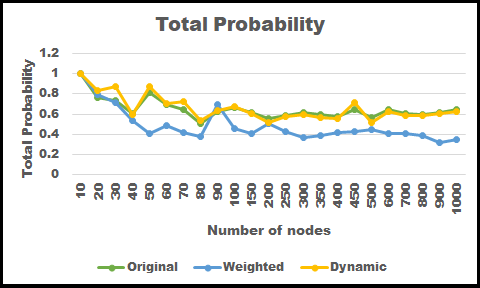
\includegraphics[width=0.6\textwidth]{Totalprob.png}\\
\caption{Line Chart of Total Probability of Original and Dynamic Probability}\\\\
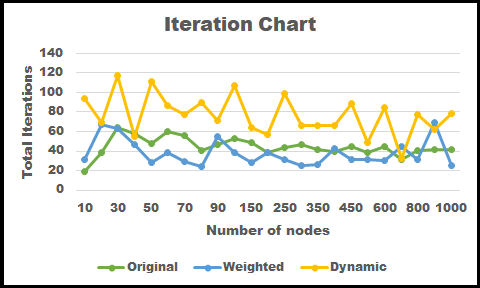
\includegraphics[width=0.6\textwidth]{iteration.png}\\
\caption{Line Chart of Total Iterations of Original and Dynamic Probability}\\
\end{center}
\section{Conclusion}
Thus we can find from this data, that the original technique can bring convergence in lesser number of iterations, Dynamic technique can be used in order to calculate the pagerank of sites, since it is close to realistic random surfer and implement probabilistic selection while surfing the sites.\\ \\
Weighted technique can also be used but pagerank tends to have varying outputs that difficult to be concluded upon. The pagerank in this method is grossly dependent in each of the weight of edges in the graph.

\section{References}
\begin{enumerate}
  \item \textbf{The Anatomy of a Large-Scale Hypertextual Web Search Engine} by Sergey Brin and Lawrence Page, \textit{Computer Science Department, Stanford University, Stanford, CA 94305}
  \item \textbf{Wikipedia} Pagerank Algorithm
  \item \textbf{Concept-based Weighted PageRank Algorithm} Bin Y Muning K. \textit{Journal of Information 2006 11: 70-72.}
  \item \textbf{Uniform Approach to Accelerated PageRank Computation} F.A. McSheary \textit{14th International Conference on World Wide Web. ACM 2005: 575-582. }
\end{enumerate}
\vspace{5cm}
\huge
\centering
-THANK YOU-
\end{document}